\chapter{Dimension reduction and Mahalanobis distance learning}
To deal with high-dimensional descriptors, dimension reduction is first performed by kernel local Fisher discriminant analysis (KLFDA). Then Mahalanobis distance metric learning based on limitations between interclass and intraclass distance is applied on dimension-reduced data.
\section{Kernel local Fisher discriminant analysis}
The extracted hierarchical Gaussian descriptors have a high dimension, and it is intractable to learn an SPD matrix with such high dimension. Dimension reduction is required to learn a subspace.
Among those methods to reduce dimension, principal component analysis (PCA) is often used. However, PCA is an unsupervised dimension reduction and may have low performance for two reasons. $(1)$, PCA is to maximize the variance of dimension-reduced data, and as an unsupervised method it doesn't take into consideration the between-class and within-class relation. It is very likely that the descriptors of different classes can be mixed up after dimension reduction. $(2)$ PCA may suffer from the small sample size problem. In some Re-ID datasets, there may be one or two images for each pedestrian in each viewpoint (like VIPeR). If the dimension of the descriptor is much bigger than the sample size, information can be lost with PCA. In this thesis, the kernel local Fisher discriminant analysis (KLFDA) is used to reduce dimension. 

KLFDA is the kernel version of LFDA, and LFDA is a combination of the Fisher discriminant analysis \cite{LFDA}, the locality preserving projection \cite{LPP} and the kernel method. A brief introduction of the FDA, LPP and kernel method is given below.
\subsection{Fisher discriminant analysis (FDA)}

FDA is a supervised dimension reduction, and its input contains the class labels. Given a set of $d$-dimensional observations $\bm{X} = (\bm{x}_1, \bm{x}_2,\cdots,\bm{x}_i,\cdots,\bm{x}_n)$, where $i\in\{1,2,\cdots,n\}$, the label $y_i\in\{1,2,\cdots,l\}$, for each sample descriptor $\bm{x}_i$, a linear transformation with transformation matrix $\bm{T}$ can be defined by the equation
\begin{equation}
\bm{z}_i = \bm{T}^T\bm{x}_i.
\end{equation}
$\bm{T}$ has a dimension of $d\times m$, and $\bm{z}_i$ is the $m(m<d)$ -dimensional vector. In FDA, two matrices are defined as the within-class scatter matrix $\bm{S}^{(w)}$ and between-class scatter matrix $\bm{S}^{(b)}$, 
\begin{equation}
\begin{aligned}
\bm{S}^{(w)} &= \mathop{\sum} _{i=1}^l\mathop{\sum}_{j:y_j = i} (\bm{x}_j - \bm{\mu}_i)(\bm{x}_j - \bm{\mu}_i)^T,\\
\bm{S}^{(b)}  &= \mathop{\sum} _{i=1}^l n_i(\bm{\mu}_i - \bm{\mu})(\bm{\mu}_i - \bm{\mu})^T,
\end{aligned}
\end{equation}
where $n_i$ is the number of classes with class label $i$, $\bm{\mu}_i$ is the mean of samples whose label is $i$, and $\bm{\mu}$ is the mean of all samples, 
\begin{equation}
\begin{aligned}
\bm{\mu}_i &= \frac{1}{n_i} \sum \bm{x}_i, \\
\bm{\mu} &= \frac{1}{n} \sum \bm{x}_i.
\end{aligned}
\end{equation}
The Fisher discriminant analysis transform matrix $\bm{T}$ can be represented as 
\begin{equation}
\bm{T} = \arg\max \frac{\bm{T}^T\bm{S}^{(b)}\bm{T}}{\bm{T}^T\bm{S}^{(w)}\bm{T}}.
\end{equation}
This equation can be solved by the Lagrange multiplier method. We define a Lagrange function as:
\begin{equation}
L(\bm{t}) = \bm{t}^T\bm{S}^{(b)}\bm{t} - \lambda(\bm{t}^T\bm{S}^{(w)}\bm{t} - 1).
\end{equation}
Then the differential respect to $\bm{t}$ is 
\begin{equation}
\frac{\partial L(\bm{t})}{\partial \bm{t}} = 2\bm{S}^{(b)}\bm{t} - 2\lambda \bm{S}^{(w)}\bm{t},
\end{equation}
let 
\begin{equation}
\frac{\partial L(\bm{t})}{\partial \bm{t}} = 0,
\end{equation}
and we can get 
\begin{equation}\label{eigen1}
\bm{S}^{(b)}\bm{t}_i  = \lambda \bm{S}^{(w)}\bm{t}_i.
\end{equation}
Here $\bm{t}_i$ is the $i_{th}$ column of $\bm{T}$, and the optimization problem is converted to an eigenvalue decomposition problem. $\bm{T}$ is the set of eigenvectors of $\frac{\bm{S}^{(b)}}{\bm{S}^{(w)}}$.

The Fisher discriminant analysis tries to minimize the intraclass scatter matrix while maximizing the interclass scatter matrix. $\bm{T}$ is computed by the eigenvalue decomposition. $\bm{T}$ can be represented as the set of all the corresponding eigenvectors, as $ \bm{T} = (\bm{t}_1,\bm{t}_2,\cdots,\bm{t}_k)$.

FDA has a form similar to signal and noise ratio; however, the FDA dimension reduction may have poor performance because it doesn't consider the locality of data. An example of this is the multimodality \cite{KLFDA}. Multimodality is when many clusters are formed in the same class. 

\subsection{Locality preserving projection (LPP)}

In \cite{LPP}, locality preserving projection (LPP) is proposed to exploit data locality. An affinity matrix is created to record the affinity of sample $\bm{x}_i$ and $\bm{x}_j$,  typically the range of elements in $\bm{A}_{i,j}$ is $[0,1]$. There are many manners to define an $n \times n$ affinity matrix $\bm{A}$; usually two sample points with a smaller distance have a higher affinity value than those with a bigger distance value. One example is that if  $\bm{x}_i$ is within k-nearest neighbours of $\bm{x}_j$, then $\bm{A}_{i,j} = 1$, otherwise  $\bm{A}_{i,j} = 0$.  

Another diagonal matrix $\bm{D}$ can be defined so that each diagonal element is the sum of the corresponding column in $\bm{A}$:
\begin{equation}
\bm{D}_{i,i} = \mathop{\sum}_{j=1}^n \bm{A}_{i, j}.
\end{equation}
Then the LPP transform matrix is defined as follow:
\begin{equation}
\bm{T}_{LPP} = \mathop{\arg\min}_{\bm{T}\in\bm{R}^{d\times m}} \frac{1}{2}\mathop{\sum}_{i, j= 1}^n \bm{A}_{i,j} ||\bm{T}^T\bm{x}_i - \bm{T}^T\bm{x}_j||,
\end{equation}
so that $ \bm{T}^T\bm{X}\bm{D}\bm{X}^T\bm{T} = \bm{I} $.
Suppose the subspace has a dimension of $m$, then the LPP transform matrix $T$ can be represented as:
\begin{equation}
\bm{T}_{LPP} = \{ \bm{\phi}_{d-m+1} | \bm{\phi}_{d-m+2} | \cdots \bm{\phi}_{d}\},
\end{equation}
and each $\bm{\phi}$ in $T$ is the eigenvector of the following formula,
 \begin{equation}
\bm{X}\bm{L}\bm{X}^T\bm{\phi} = \gamma\bm{X}\bm{D}\bm{X}^T,
\end{equation}
where $\gamma$ is corresponding eigenvalue of $\bm{\phi}$, and $\bm{L} = \bm{D} - \bm{A}$.
%where $\bm{D}$ is the $n$-dimensional diagonal matrix with $i_{th}$ diagonal element 
%\begin{equation}
%\bm{D}_{i,i} = \sum_{j = 1}^n\bm{A}_{i,j}
%\end{equation}

%But the LPP dimension reduction is still not discriminant enough, 
\subsection{Local Fisher discriminant analysis (LFDA)}
\indent LFDA \cite{LFDA} combines FDA and LPP and has better performance. The key to LFDA is that it assigns weights to elements in $\bm{A}^{(w)}$ and $\bm{A}^{(b)}$, so that
\begin{equation}
\begin{aligned}
\bm{S}^{(w)} &= \frac{1}{2}\sum _{i=1}^l\sum_{j:y_j = i} \bm{A}_{i,j}^w (\bm{x}_j - \bm{\mu}_i)(\bm{x}_j - \bm{\mu}_i)^T,\\
\bm{S}^{(b)} &=  \frac{1}{2}\sum _{i=1}^l \bm{A}_{i,j}^b(\bm{\mu}_i - \bm{\mu})(\bm{\mu}_i - \bm{\mu})^T,
\end{aligned}
\end{equation}
where 

\begin{equation}
\begin{aligned}
\bm{A}_{i,j}^{(w)} = \left \{ 
\begin{array}{rcl}
\bm{A}_{i,j}/n_c &  &y_i = y_j \\
0 & & {y_i \ne y_j }
\end{array}
  \right. , \\
  \bm{A}_{i,j}^{(b)} = \left \{ 
\begin{array}{rcl}
(\frac{1}{n} - \frac{1}{n_c})  \bm{A}_{i,j} &  &{y_i = y_j }\\
\frac{1}{n} & & {y_i \ne y_j }
\end{array}
  \right. ,
 \end{aligned}
\end{equation}
where $y_i$ is the class label of sample point $\bm{x}_i$. So the transformation matrix $T_{LFDA}$ can be computed by the equation
\begin{equation}\label{eigencompute1} 
\bm{T}_{LFDA}  = \arg\min_{\bm{T}} (\frac{\bm{T}^T\bm{S}^{(b)}\bm{T}}{\bm{T}^T\bm{S}^{(w)}\bm{T}}).
\end{equation}
Again, this problem can be solved by eigenvalue decomposition with Equation \ref{eigen1}. 



When applying the LFDA to original high-dimensional descriptors, one problem is the computational cost. Suppose the vector data has a dimension of $d$, then LFDA has to solve the eigenvalues of a matrix with a dimension $d\times d$. In some descriptors, $d$ could be more than 20000 and the computation cost is intractable. 
 
\subsection{Kernel local Fisher discriminant analysis (KLFDA)}

KLFDA  \cite{KLFDA} is the nonlinear version of LFDA. Most dimensionality reduction methods, including PCA, LDA and LFDA, are linear dimensionality reduction methods. However, when descriptor data is non-linear in feature space, it's hard to capture its between-class discriminant information with linear reduction methods. One alternative method is to nonlinearly map input descriptors $\bm{x}_i$ to higher-dimensional feature space $\Phi$ by a function $\phi(\bm{x}_i)$. Again, the LFDA is performed in feature space $\Phi$. Thus the transformation matrix $\bm{T}$ can be computed by the equation
\begin{equation}
\bm{T} = \arg \min \frac{\bm{T}^T\bm{S}^{(b)}_{\phi}\bm{T}}{\bm{T}^T\bm{S}^{(w)}_{\phi}\bm{T}},
\end{equation}
where $\bm{S}^{(b)}_{\phi}$ and $\bm{S}^{(w)}_{\phi}$ is the between-class scatter and within-class scatter in mapped feature space $\Phi$.

Note that with the transformation matrix $\bm{T} \in \Phi$, it is computationally expensive to explicitly compute the mapping function $\phi$ and perform LFDA in feature space $\Phi$ because the dimension of $\Phi$ may be infinite. Rather than explicitly computing, the mapping function $\phi$ can be implicit, and the feature space $\Phi$ can be defined by the inner product of features in $\Phi$. The kernel trick is used here, and a kernel function can be defined as the inner product of mapped vectors $\phi(\bm{x}_i)$ and $\phi(\bm{x}_j)$ by the equation
 \begin{equation}
 k(\bm{x}_i,\bm{x}_j) = <\phi(\bm{x}_i),\phi(\bm{x}_j)>,
 \end{equation}
where the $< \cdot >$ is the inner product. There are many kinds of kernels like the linear kernel, the polynomial kernel and the radial basis function (RBF) kernel. In this paper, the RBF kernel is adopted. An RBF kernel is defined as 
 \begin{equation}
 k_{RBF}(\bm{x}_i,\bm{x}_j) = \exp^{(-\gamma||\bm{x}_i-\bm{x}_j||^2)}. 
 \end{equation}
Suppose $\bm{X}$ is the matrix of sample descriptors, and we have
\begin{equation}
\bm{X} = (\bm{x}_1, \bm{x}_2,\cdots, \bm{x}_n), 
\end{equation}
and the label vector is $\bm{l} = (l_1, l_2, \cdots, l_n)$. Then the kernel matrix of $\bm{X}$ can be computed as the following equation:
\begin{equation}
\bm{K} =  \phi(\bm{X})^T \phi(\bm{X}),
\end{equation}
and we have 
\begin{equation}
\bm{K}_{i,j} =  k(\bm{x}_i,\bm{x}_j) = <\phi(\bm{x}_i),\phi(\bm{x}_j)> =  \exp^{(-\gamma||\bm{x}_i-\bm{x}_j||^2)}.
\end{equation}
In \cite{KLFDA}, the authors proposed fast computation of LFDA by replacing $\bm{S}^{(b)}$ with the local scatter mixture matrix $\bm{S}^{(m)}$defined by 
\begin{equation}
\begin{aligned}
\bm{S}^{(m)} &= \bm{S}^{(b)} + \bm{S}^{(w)},\\
\bm{S}^{(m)} &= \frac{1}{2} \sum_{i,j = 1} \bm{A}_{i,j}^{(m)} (\bm{x}_i - \bm{x}_j)(\bm{x}_i - \bm{x}_j)^T,
\end{aligned}
\end{equation}
and 

\begin{equation}
\bm{A}_{i,j}^{(m)} = \bm{A}_{i,j}^{(w)}  + \bm{A}_{i,j}^{(w)}.
\end{equation}

\noindent According to the identity (cf. (Fukunaga, 1990))
\begin{equation}
trace((\bm{T}^T\bm{S}^{(w)}\bm{T})^{(-1)}(\bm{T}^T\bm{S}^{(m)}\bm{T}) = trace((\bm{T}^T\bm{S}^{(w)}\bm{T})^{(-1)}(\bm{T}^T\bm{S}^{(b)}\bm{T}) + m.
\end{equation}
Equation \ref{eigencompute1} is equal to 

\begin{equation}
\bm{T}_{LFDA}  = \arg\min_{\bm{T}} (\frac{\bm{T}^T\bm{S}^{(m)}\bm{T}}{\bm{T}^T\bm{S}^{(w)}\bm{T}}),
\end{equation}
and it can be transformed into a eigenvalue decomposition problem 
\begin{equation}\label{eigen2}
\bm{S}^{(m)}\bm{t}_i  = \lambda \bm{S}^{(w)}\bm{t}_i.
\end{equation}
With the replacement of $\bm{S}^{(m)}$, in \cite{KLFDA} the author summarized that 
\begin{equation}
\bm{S}^{(m)} = \bm{X}\bm{L}^{(m)}\bm{X}^T,
\end{equation}
where $\bm{L}^{(m)}  = \bm{D}^{(m)} - \bm{A}^{(m)}$, and $ \bm{D}^{i,i} = \sum_{j=1}^n  \bm{A}_{i,j}^{(m)}$. Also, $\bm{S}^{(w)}$ can be represented as 
\begin{equation}
\bm{S}^{(w)} = \bm{X}\bm{L}^{(w)}\bm{X}^T,
\end{equation}
where $\bm{L}^{(w)}  = \bm{D}^{(w)} - \bm{A}^{(m)}$, and $ \bm{D}^{i,i} = \sum_{j=1}^n  \bm{A}_{i,j}^{(w)}$. 
Therefore, Equation \ref{eigen2} can be represented as
\begin{equation}\label{equationS}
\bm{X}\bm{L}^{(m)}\bm{X}^T \bm{t}_i= \lambda\bm{X}\bm{L}^{(w)}\bm{X}^T \bm{t}_i.
\end{equation}
The eigenvector $\bm{t}_i$  can be represented as $\bm{t}_i = \bm{X}\bm{\gamma}$, vector $\bm{\gamma}_i \in R^n$. With this replacement, we left multiply $\bm{X}^T$ to Equation \ref{equationS} to get 
\begin{equation}
\bm{X}^T\bm{X}\bm{L}^{(m)}\bm{X}^T\bm{X}\gamma_i = \lambda\bm{X}^T\bm{X}\bm{L}^{(w)}\bm{X}^T \bm{X}\gamma_i,
\end{equation}
and with the kernel trick, it's represented as
\begin{equation}
\bm{K}\bm{L}^{(m)}\bm{K}\gamma_i  = \lambda \bm{K}\bm{L}^{(w)}\bm{K}\gamma_i.
\end{equation}
One example of using KLFDA to reduce dimension and classify the nonlinear data clusters can be shown in Figures \ref{KLFDAdemo1}, \ref{KLFDAdemo2} and \ref{KLFDAdemo3}. Three classes with five clusters are distributed on a 2D plane, and by KLFDA dimension reduction their 1D dimension-reduced data distribution are shown in Figure \ref{KLFDAdemo2} and Figure \ref{KLFDAdemo3}. We can conclude that for those clusters the Gaussian kernel is better than the linear kernel because the dimension-reduced data is more separate when using Gaussian kernel function.

\begin{figure}[H]
\centering
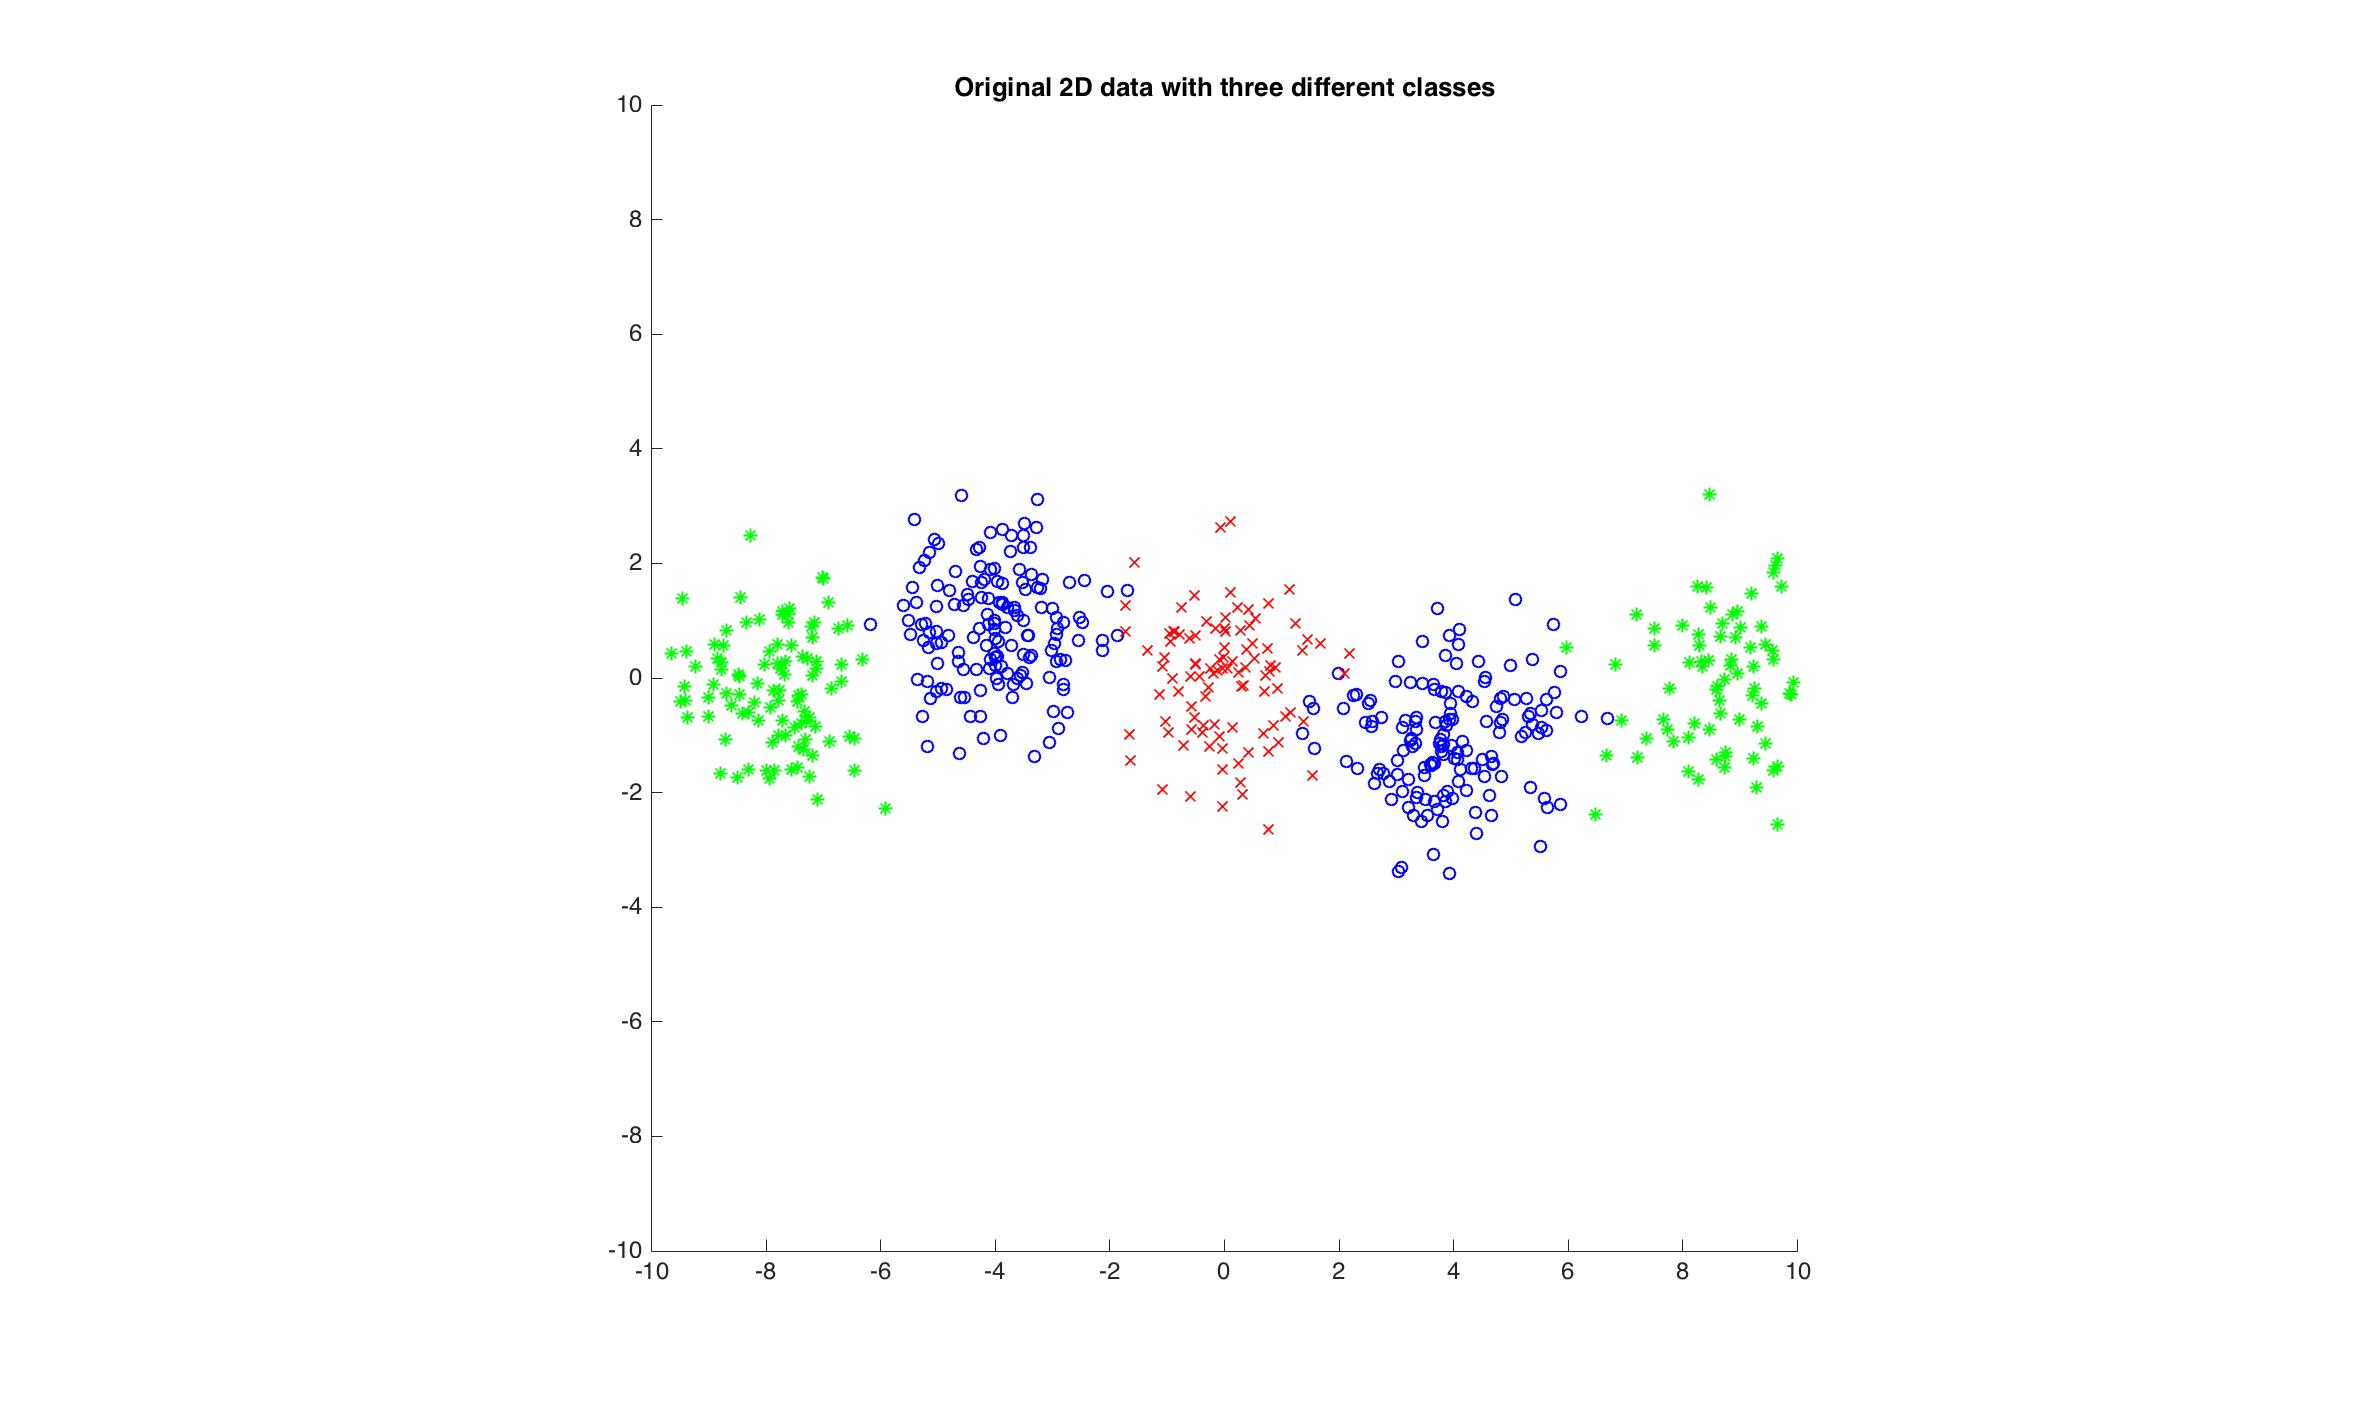
\includegraphics[width=1\linewidth]{/Users/JohnsonJohnson/Downloads/thesis_1/Figures/KLFDAdemo1.jpg}
\caption{Example of five clusters that belong to three classes}
\label{KLFDAdemo1}
\vspace{-1em}
\end{figure} 


\begin{figure}[H]
\centering
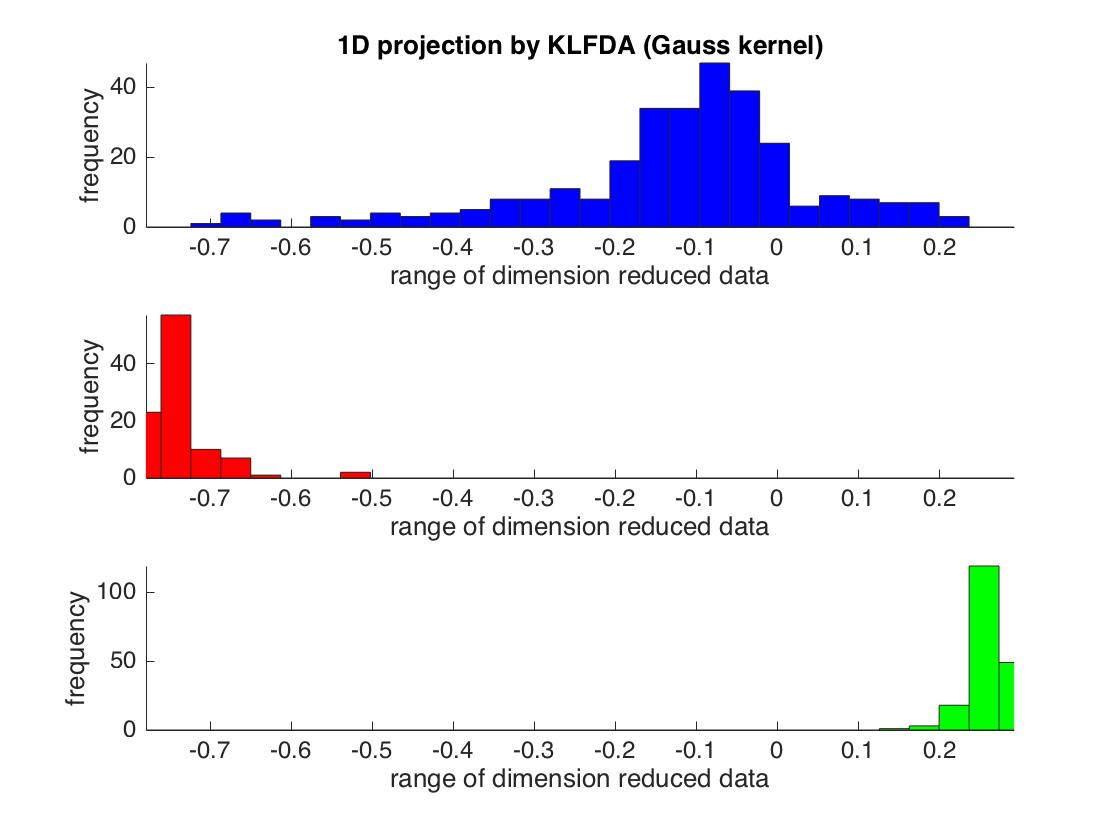
\includegraphics[width=1\linewidth]{/Users/JohnsonJohnson/Downloads/thesis_1/Figures/KLFDAdemo2.jpg}
\caption{1D distribution of dimension-reduced data with Gaussian kernel}
\label{KLFDAdemo2}
\vspace{-1em}
\end{figure} 


\begin{figure}[H]
\centering
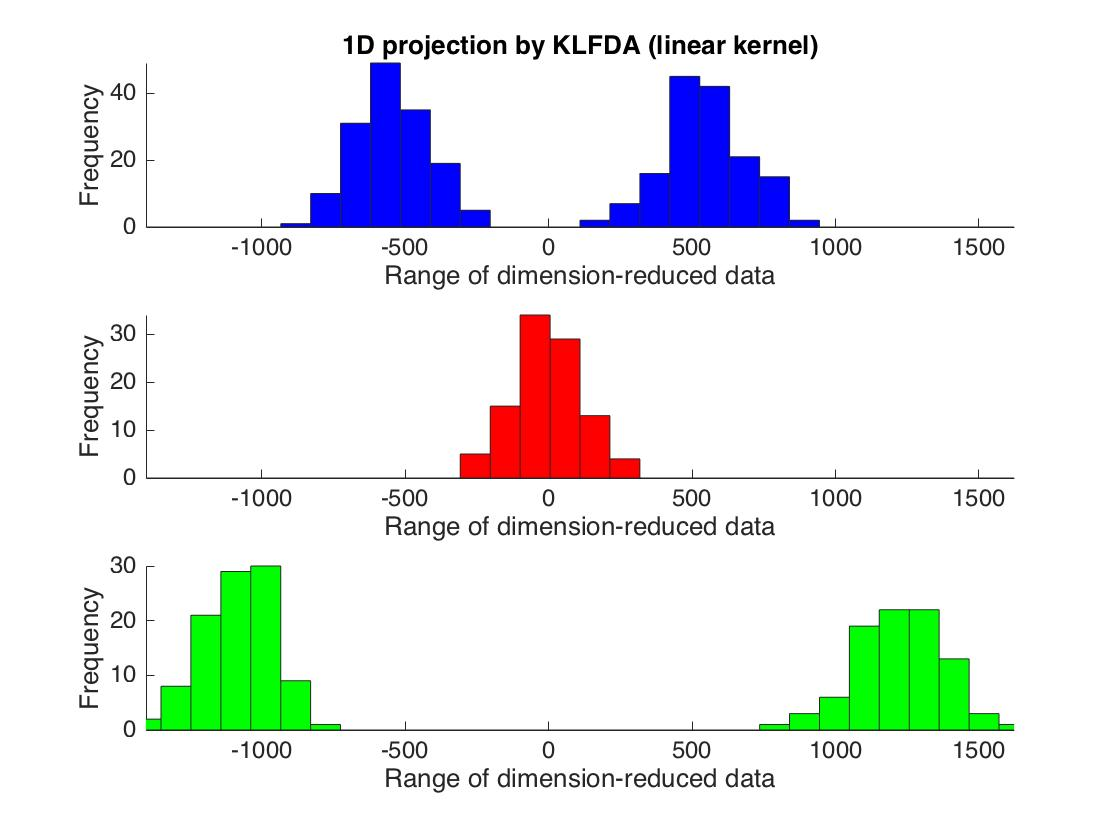
\includegraphics[width=1\linewidth]{/Users/JohnsonJohnson/Downloads/thesis_1/Figures/KLFDAdemo3.jpg}
\caption{1D distribution of dimension-reduced data with linear kernel}
\label{KLFDAdemo3}
\vspace{-1em}
\end{figure} 

%\begin{figure}[H]
%\centering
%\begin{minipage}[t]{0.5\linewidth}
%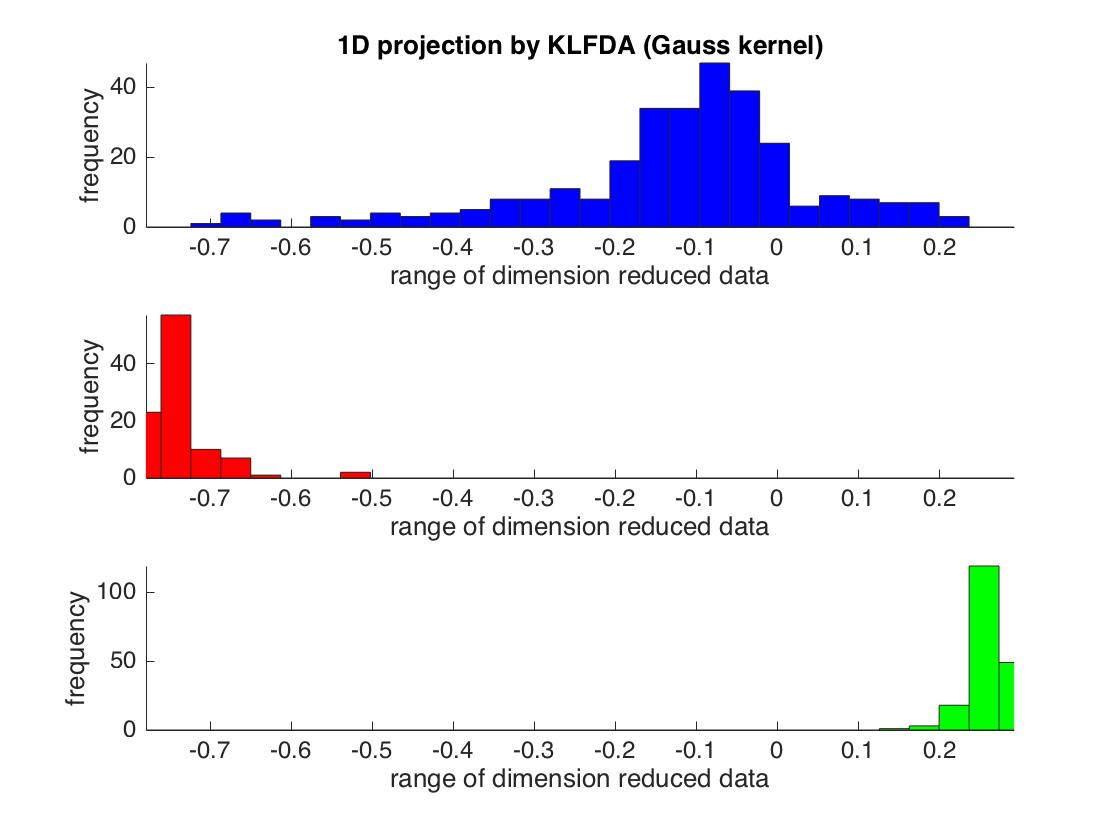
\includegraphics[width=2.7in]{/Users/JohnsonJohnson/Downloads/thesis_1/Figures/KLFDAdemo2.jpg}
%%\caption{RGB patch}
%\label{fig:side:a}
%\end{minipage}%
%\begin{minipage}[t]{0.5\linewidth}
%\centering
%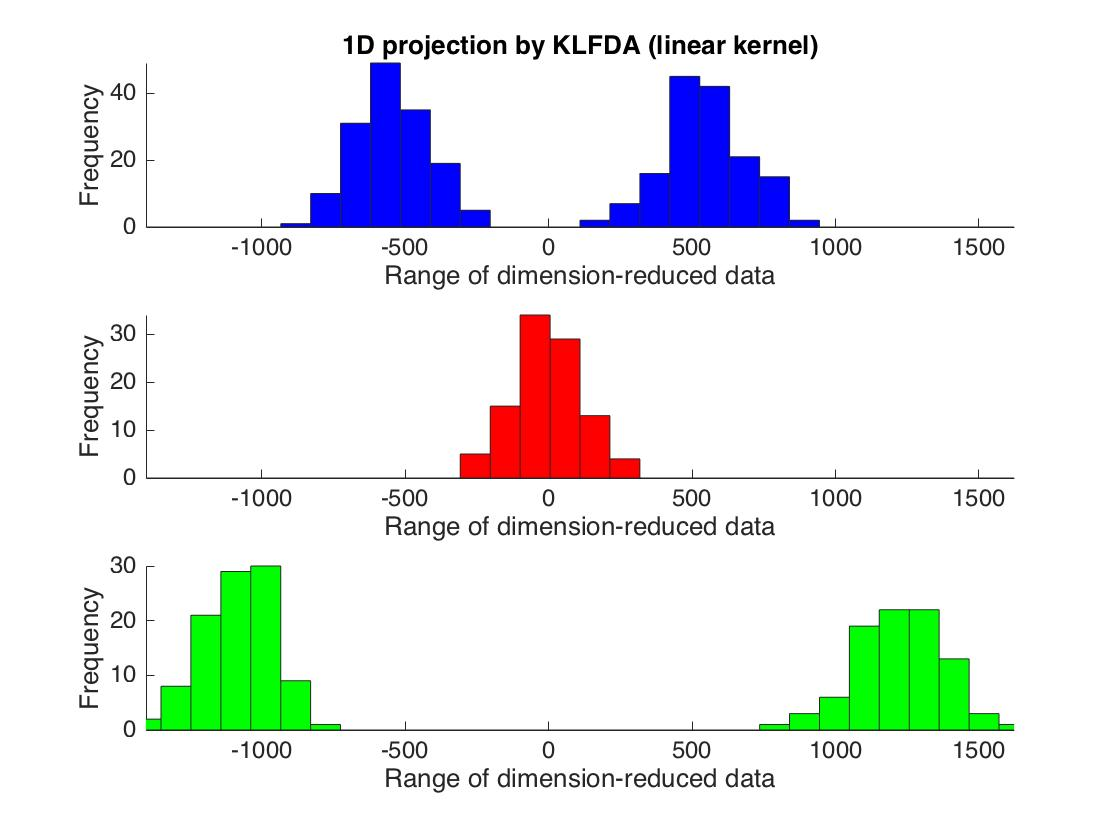
\includegraphics[width=2.7in]{/Users/JohnsonJohnson/Downloads/thesis_1/Figures/KLFDAdemo3.jpg}
%%\caption{GBR patch}
%\label{fig:side:b}
%\end{minipage}
%\caption{A comparison of two patches with same entropy but different color distribution}
%\end{figure}

\section{Mahalanobis distance}
Mahalanobis distance \cite{Mahadist} based metric learning has received much attention in similarity computing. The Mahalanobis distance of two observations $\bm{x} $ and $\bm{y}$ is defined as
\begin{equation}
\label{MahaDist}
D(\bm{x},\bm{y}) = (\bm{x} - \bm{y})^T\bm{M}(\bm{x} - \bm{y}), 
\end{equation}
where $\bm{x}$ and $\bm{y} $ are $d\times1$-dimensional observation vectors, and $\bm{M}$ is a semi-positive definite matrix. Since $\bm{M}$ is an SPD matrix, $\bm{M}$ can be decomposed as $\bm{M} = \bm{W}^T\bm{W}$, and the Mahalanobis distance can also be written as 
\begin{equation}
D(\bm{x},\bm{y}) = (\bm{x} - \bm{y})^T\bm{W}^T\bm{W}(\bm{x} - \bm{y})= ||\bm{W}(\bm{x} - \bm{y})||.
\end{equation}
 Therefore, Mahalanobis distance can be regarded as a variant of Euclidean distance.
 
 \section{Gradient descent optimization}
 Given a multivariate function $F(\bm{x})$, where $\bm{x}$ is a $d$-dimensional vector, if $f(\bm{x})$ is continuous and differentiable in the neighbour of point $\bm{x}$ for all $\bm{x}$, then $f(\bm{x})$ decreases fastest toward the direction of the negative gradient of $F(\bm{x})$. To compute the minimum of $F(\bm{x})$, an iterative method can be used by updating $F$ with respect to $\bm{x}$. If the updating step $\lambda$ is small enough, by updating $\bm{x}$ with 
 \begin{equation}
 \bm{x}_{t+1} = \bm{x}_{t} - \lambda \bm{G},
 \end{equation}
we have 
  \begin{equation}
 F(\bm{x}_{t+1}) \ge F(\bm{x}_t).
  \end{equation}
This process is repeated until a certain condition is met, generally when gradient $||\bm{G}|| \le \eta$, and $\eta$ is a very small positive integer. 
\begin{figure}
\centering
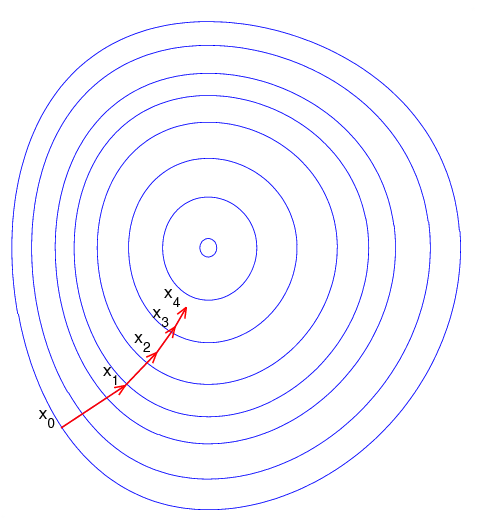
\includegraphics[width=0.4\linewidth]{/Users/JohnsonJohnson/Downloads/thesis_1/Figures/Gradientdescent.png}
\caption{Steepest gradient descent}
\vspace{0em}
\end{figure} 

\textbf{Analysis of steepest gradient descent method} The advantages of gradient descent are that it is always downhill and it can avoid the saddle points. Besides, it is very efficient when the initial value of $F(\bm{x})$ is far from the minimum. However, there are a few shortcomings of the gradient descent method. The first one is that the convergence value of gradient descent might be the local minima of $F(\bm{x})$ if $F(\bm{x})$ is not monotonic. In this case, the convergence value will depend on the initial value of $\bm{x}$. Another shortcoming is that the converging speed goes very slowly when approaching the minimum. One example is the case of zigzag downhill. The third shortcoming is linear search in gradient descent might cause some problems.
%\begin{figure}[H]
%\begin{minipage}[t]{0.5\linewidth}
%\centering
%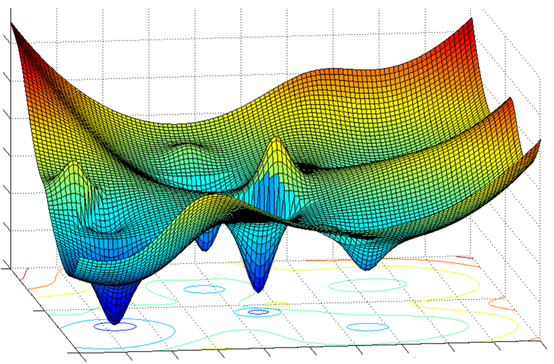
\includegraphics[width=2.2in]{/Users/JohnsonJohnson/Downloads/thesis_1/Figures/multiMinima.png}
%\caption{Function with multi local minimums}
%\label{fig:side:a}
%\end{minipage}%
%\begin{minipage}[t]{0.5\linewidth}
%\centering
%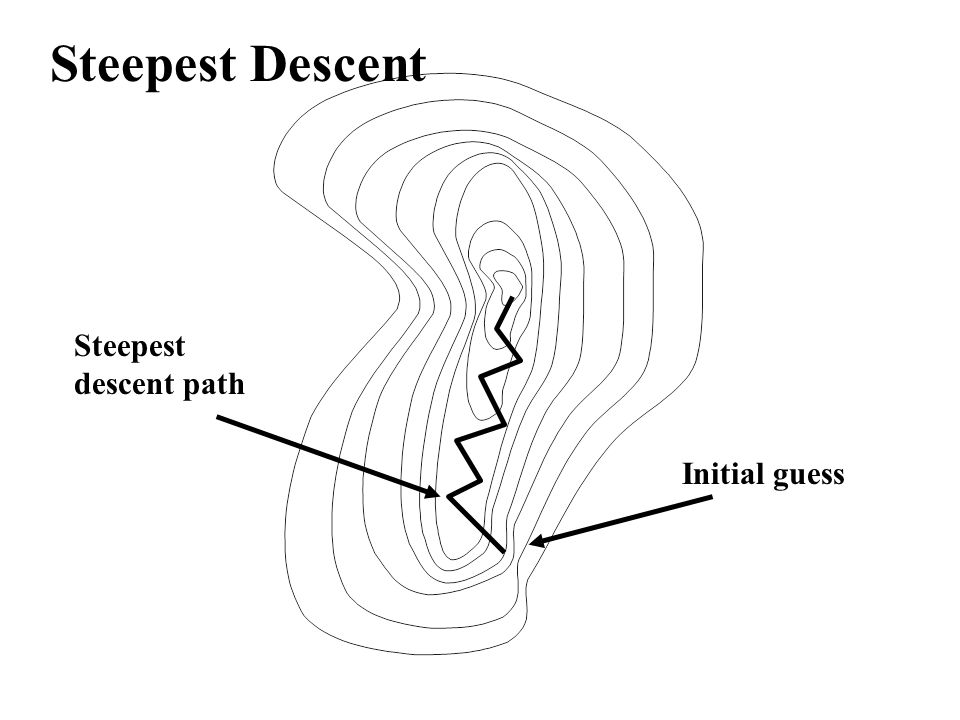
\includegraphics[width=2.2in]{/Users/JohnsonJohnson/Downloads/thesis_1/Figures/zigzag.jpg}
%\caption{Zigzagging downhill valley}
%\label{fig:side:b}
%\end{minipage}
%\end{figure}

 \section{Metric learning based on sample pairs distance comparison}
 Inspired by \cite{TDL}, a similar metric learning based on iteration computation is used. For a  sample descriptor $\bm{x}_i$,  its positive pairwise set is defined as $\{\bm{x}_i,\bm{x}_j\}$, where class ID $y_i = y_j$. Also, the negative pairwise set can be defined as $\{\bm{x}_i,\bm{x}_j\}$, where $y_i \ne y_j$. Similarly, the method in \cite{PRDC} is also based on similarity comparison. In \cite{PRDC}, for all possible positive and negative pairs, the distance between positive pairs must be smaller than the distance between negative pairs. Since it has to compare all possible positive and negative pairs, its computation complexity is quite expensive. To reduce the complexity, a simplified version is proposed as the top-push distance metric learning \cite{TDL}.  Since re-identification is a problem of ranking, it is desired that the rank-1 descriptor should be the right match. Given a Mahalanobis matrix $\bm{M}$, for samples $\bm{x}_i, i = 1,2,3,\cdots,n$, where $n$ is the number of all the samples, the requirement is that the maximum distance among all positive pairs should be at least one unit smaller than the minimum distance of all negative pairs. This can be denoted as 
 \begin{equation}
 D(\bm{x}_i,\bm{x}_j) + \rho < \min D(\bm{x}_i,\bm{x}_k), y_i = y_j, y_i\ne y_k,
 \end{equation}
 where $\rho$ is a slack variable and $\rho \in [0,1]$. This equation can be transformed into an optimization problem as
 \begin{equation}
 \label{term1}
 \min \sum_{y_i = y_j} \max \{D(\bm{x}_i,\bm{x}_j) -  \min_{ y_i\ne y_k} D(\bm{x}_i,\bm{x}_k)  + \rho , 0\}.
 \end{equation}
However, the equation above only penalizes the minimum interclass distance. Another term is needed to penalize large intraclass distance. That is, the sum of intraclass distance should be as small as possible. This term is denoted as 
 \begin{equation} \label{term2}
 \min \sum_{y_i = y_j} D(\bm{x}_i,\bm{x}_j).
 \end{equation}

 
 To combine the equations above, a ratio factor $\alpha$ is assigned to Equation \eqref{term1} and \eqref{term2} so that the target function can be denoted as 
  \begin{equation}
  \label{TargetFunc1}
  \begin{aligned}
 f(\bm{M}) = (1-\alpha)\sum_{\bm{x}_i,x_j,\bm{y}_i=y_j} D(\bm{x}_i,\bm{x}_j) + \\
  \alpha \sum_{\bm{x}_i,\bm{x}_j,y_i=y_j}\max\{{D(\bm{x}_i,\bm{x}_j)-\min_{y_i\ne y_k}{D(\bm{x}_i,\bm{x}_k)}+\rho,0}\}.
 \end{aligned}
 \end{equation}
 In this way, the problem is transformed to an optimization problem. Notice that Equation \ref{MahaDist} can be denoted as 
 \begin{equation}
 D(\bm{x},\bm{y}) = (\bm{x} - \bm{y})^T\bm{M}(\bm{x} - \bm{y}) = trace(\bm{M}\bm{X}_{i,j}),
 \end{equation}
 where $\bm{X}_{i,j} = \bm{x}_i*\bm{x}_j^T$, and $trace$ is to compute the matrix trace. Therefore, Equation \ref{TargetFunc1} can be transformed as follows:
 \begin{equation}
 \label{TargetFunc2}
 \begin{aligned}
 f(\bm{M}) = (1-\alpha)\sum_{y_i = y_j}trace(\bm{M}\bm{X}_{i,j}) \\
  + \alpha \sum_{y_i = y_j,y_i\ne y_k}\max\{trace(\bm{M}\bm{X}_{i,j}) - trace(\bm{M}\bm{X}_{i,k} )+ \rho,0\}.
 \end{aligned}
 \end{equation}
 
 To minimize Equation \ref{TargetFunc2}, the gradient descent method is used. The gradient respect to $\bm{M}$ is computed as
 \begin{equation}
 \begin{aligned}
\bm{G} =  \frac{\partial f}{\partial \bm{M}} = (1-\alpha) \sum_{y_i = y_j} \bm{X}_{i,j} 
 + \alpha \sum_{y_i = y_j, y_i \ne y_k}(\bm{X}_{i,j} - \bm{X}_{i,k}).
 \end{aligned}
 \end{equation}
 
 The iteration process can be summarized in Table \ref{Gradientdemo}.
% \begin{table}[H]
% \caption{The optimization algorithm for metric learning}
% \centering
% \begin{tabular}{l}
% \hline 
% \multicolumn{1}{l}{\textbf{Gradient optimization algorithm for target function}} \\
% \hline
% \textbf{Input} Descriptors of training person pairs \\
% \textbf{Output} A SPD matrix\\
% \textbf{Initialization} \\
% Initialize $\bm{M}$ with eye matrix $\bm{I}$; \\
% Compute the initial target function value $f_0$ with $\bm{M}_0$;\\
% Iteration count  $t = 0$;\\
%
% \textbf{while}(not converge)\\
% \space Update $t =  t + 1$;\\
% \indent Update gradient $\bm{G}_{t+1}$ with equation 24;\\
% \indent Update $\bm{M}$ with equation : $\bm{M}_{t+1} = \bm{M}_{t} - \lambda\bm{G}_t$\\
% \indent Project $\bm{M}_{t+1}$ to the positive semi-definite space \\ 
% \indent \indent by $\bm{M}_{t+1}= \bm{V}_{t+1}\bm{S}_{t+1}\bm{V}^T_{t+1}$;\\
% \indent Update the target value $f|_{\bm{M} = \bm{M}_{t+1}}$;\\
% \textbf{end while}  \\
% return $\bm{M}$\\
% \hline
% \end{tabular} 
% \end{table}
In each iteration, to make sure the updated $\bm{M}$ is an SPD matrix, first a eigenvalue decomposition is performed on $\bm{M}$, and we have
\begin{equation}\label{SPDproject}
\bm{M} = \bm{V}\bm{\Lambda}\bm{V}^T.
\end{equation}
Here $\bm{\Lambda}$ is a diagonal matrix, and its diagonal elements are eigenvalues. Then the negative eigenvalues in $\bm{V}$ are removed, and the corresponding eigenvectors in $\bm{V}$ are also removed. Then $\bm{M}$ is restored by Equation \eqref{SPDproject}.

\begin{table}[H]
 \centering
 \caption{Optimization algorithm of Mahalanobis distance matrix learning}
 \label{Gradientdemo}
 \begin{tabular}{l}
 \hline 
 \multicolumn{1}{l}{\textbf{Gradient optimization algorithm for target function}} \\
 \hline
 \textbf{Input} Descriptors of training person pairs \\
 \textbf{Output} An SPD matrix\\
 \textbf{Initialization} \\
 Initialize $\bm{M}_0$ with eye matrix $\bm{I}$; \\
 Compute the initial target function value $f_0$ with $\bm{M}_0$;\\
 Iteration count  $t = 0$;\\

 \textbf{while}(not converge)\\
 \hspace{0.5cm} Update $t =  t + 1$;\\
 \hspace{0.5cm}  Find $\bm{x}_k$ for all sample points $\bm{x}_i$, where $y_i \ne y_k$;\\
 \hspace{0.5cm} Update gradient $\bm{G}_{t+1}$ with Equation 12;\\
 \hspace{0.5cm}  Update $\bm{M}$ with equation : $\bm{M}_{t+1} = \bm{M}_{t} - \lambda\bm{G}_t$;\\
 \hspace{0.5cm}  Project $\bm{M}_{t+1}$ to the positive semi-positive definite space; \\ 
% \indent \indent by $\bm{M}_{t+1}= \bm{V}_{t+1}\bm{S}_{t+1}\bm{V}^T_{t+1}$;\\
 \hspace{0.5cm}  Update the target value $f|_{\bm{M} = \bm{M}_{t+1}}$;\\
 \textbf{end while}  \\
 return $\bm{M}$\\
 \hline
 \end{tabular} 
 \end{table}
 
 
 
 
 
